
%\chapter*{A brief introduction to quantum field theory in curved spacetimes: Introduction to the Unruh and Hawking effects}[Intro to the Unruh and Hawking effects]
%\label{chap:introUnruh}


\chapter[Introduction to QFT in curved spacetimes]{Introduction to quantum field theory in curved spacetimes}\label{INTROU}

This  section of the preliminars pursuits a double objective. First, it aims to give a brief introduction to the tools and the background of quantum field theory in curved spacetimes necessary to understand and to present the results obtained during the development of this thesis. Of course this is only a very brief introduction to a very complex and extense discipline, more thorough approaches to these topics can be found in many textbooks \cite{Wald2,Birrell,NavarroSalas}

Second, in section \ref{probexcitations} we analyse a problem present in most of the previous literature, the use of the `single mode approximation' introduced in \cite{Alsingtelep,AlsingMcmhMil} based on misleading assumptions. In this section we will introduce new material which will be necessary in order to discuss the new work presented in part \ref{part1} in the context of previous results in the literature, giving a correct interpretation for this approximation. However, it will be in chapter \ref{sma} when this topic will be thoroughly dealt with when we expose the new results obtained when going beyond such approximation. 

\section{Scalar field quantisation in Minkowski \mbox{spacetime}}\label{scalarfieldq}

In this section I present a brief review of the standard canonical quantisation procedure of a field in Minkowski spacetime. The aim of this section is to introduce the concepts and notation that are going to be used throughout the following sections. Therefore, for the sake of simplicity, we will focus on a real massless scalar field. 

Let us consider an inertial observer (Alice) of the flat spacetime whose proper coordinates are the Minkowskian coordinates $(t,x, y, z)$. She wants to build a quantum field theory for a free masless scalar field. 

The equation of motion for this field is the well-known Klein-Gordon equation in Minkowski coordinates
\begin{equation}\label{KG1}
(\Box -m^2)\Phi =0.
\end{equation}

As it is commonplace, we can expand an arbitrary solution $\Phi(\bm x,t)$ to this equation as a sum of `positive frequency' and `negative frequency' solutions. One could innocently ask what is the definition of positive and negative frequency solutions, but the answer is somewhat trivial if we work with the Minkowski spacetime as background. The Minkowski spacetime admits a global timelike Killing vector $\partial_t$. A positive frequency solution of \eqref{KG1} $u_k(\bm x,t)$ satisfies, therefore,
\begin{equation}\label{flatcriterion}
\partial_t u_k(\bm x,t)=-i\omega_ku_k(\bm x,t),
\end{equation}
and this criterion would be the same if instead of $t$ we use the proper time of any inertial observer. Hence, we will express  $\Phi(\bm x,t)$ as a combination of positive $u_i(\bm x,t)$ and negative  $u^*_i(\bm x,t)$ frequency solutions of \eqref{KG1} with respect to Alice's proper time\footnote{For notational convenience we are using the sum symbol $\sum_i$ meaning integration over frequencies. Note that in free space $\sum_i\rightarrow\int_{-\infty}^\infty \frac{d^Dk}{\sqrt{(2\pi)^d2\omega}}$ and the modes are normalised to Dirac's delta instead of Kronecker's delta} and her definition will agree  with the definition of any other inertial observer.
\begin{equation}\label{exp1}
\Phi(\bm x,t)=\sum_i \left[\alpha_i u_i(\bm x,t)+\alpha_i^* u^*_i(\bm x,t)\right].
\end{equation}

The solutions $u_i(\bm x,t)$ can be chosen to form an orthonormal basis of solutions with respect to the Klein-Gordon scalar product defined, through the continuity equation, as
\begin{equation}\label{KGsc}
(u_j,u_k)=-i\int \text{d}^3x\left(u_j\partial_tu_k^*-u_k^*\partial_tu_j\right),
\end{equation}
which on the space of positive energy solutions happens to be positive definite. Note that, obviously, the modes $u_j$ satisfy the orthonormality relations
\begin{equation}\label{orto}
(u_j,u_k)=\delta_{jk}=-(u_j^*,u_k^*),\qquad (u_j,u_k^*)=0.
\end{equation}
We can now construct a Fock space following the standard canonical field quantisation scheme.

First we promote the classical Klein-Gordon field to a quantum field operator satisfying the equal time commutation relations
\begin{equation}
\begin{array}{c}
\left[\Phi(\bm x,t),\Pi(\bm x',t)\right]=i\delta(\bm x-\bm x'),\\[3mm]
\left[\Phi(\bm x,t),\Phi(\bm x',t)\right]=\left[\Pi(\bm x,t),\Pi(\bm x',t)\right]=0,
\end{array}
\end{equation}
where $\Pi(\bm x,t)=\partial_t \Phi(\bm x,t)$ is the canonical conjugate momentum associated with the variable $\Phi$.

This promotion means that we have to replace the complex amplitudes $\alpha_i$ and $\alpha_i^*$ by annihilation and creation operators $a_i$ and $a_i^\dagger$ who inherit the following commutation relations
\begin{equation}
\begin{array}{c}
[a_i,a^\dagger_j]=(u_i,u_j)=\delta_{ij},\\[3mm]
[a_i,a_j]=[a^\dagger_i,a^\dagger_j]=0.
\end{array}
\end{equation}

Now we can construct the standard Fock space, first we characterise the vacuum state of the field (minimum energy state) as the state which is annihilated by all the operators $a_i$
\begin{equation}
a_i\ket{0}=0.
\end{equation}

Then we define the one-particle Hilbert space by applying the creation operators $a_i^\dagger$ on the vacuum state
\begin{equation}
\ket{1_i}=a^\dagger_i\ket{0},
\end{equation}
and so on and so forth we construct the complete Fock space
\begin{equation}
\ket{n^1_{i_1},n^2_{i_2},\dots,n^k_{i_k}}=\frac{1}{\sqrt{n^1!n^2!\dots n^k!}} (a^\dagger_{i_1})^{n^1}(a^\dagger_{i_2})^{n^2}\dots(a^\dagger_{i_k})^{n^k}\ket{0}.
\end{equation}

Note that this quantisation procedure is independent of the particular choice of the inertial observer Alice. Any other choice of time $t$ is related to this one via Poincar\'e transformations which do not modify what we would label as positive and negative frequency modes. As a consequence, the expansion \eqref{exp1} can be performed equivalently for any inertial reference frame and the splitting between positive and negative frequency modes is invariant. Hence, the vacuum state is also Poincar\'e invariant and the construction of the Fock space is equivalent for any inertial observer. This will not happen for a general spacetime, as we will see in the following sections.

\section{Field quantisation in curved spacetimes}

For general spacetimes we cannot assume that we have global Poincar\'e symmetry and we will run into many difficulties when trying to construct quantum fields.

Let us continue with the scalar field case for the sake of simplicity. First of all we generalise equation \eqref{KG1} by means of the covariant D'Alambert operator, obtained promoting the partial derivatives to the covariant derivatives $\Box =\partial_\mu\partial^\mu\rightarrow \nabla_\mu\nabla^\mu$ so that  equation\footnote{There are some subtleties that should not be overlooked: first of all, we are assuming that there is no coupling of the field with the scalar curvature (minimal coupling). Second of all, if the field had internal spin degrees of freedom one must be careful with the covariant derivative definition (See Appendix \ref{appB})} \eqref{KG1} now reads
\begin{equation}
\nabla_\mu\nabla^\mu \phi =0.
\end{equation}
 
 To extend the Klein-Gordon product \eqref{KGsc} to curved spacetime we need a complete set of initial data, in other words, a Cauchy hypersurface $\Sigma$ over which we have to extend the integral\footnote{It can be shown, using Gauss theorem, that the product is independent of the choice of the Cauchy hypersurface $\Sigma$}
 \begin{equation}\label{KGscc}
(u_j,u_k)=-i\int \text{d}\Sigma\, n^\mu\left(u_j\partial_\mu u_k^*-u_k^*\partial_\mu u_j\right),
 \end{equation}
where $d\Sigma$ is the volume element and $n^\mu$ is a future directed timelike unit vector which is orthogonal to $\Sigma$.

Whether the spacetime is stationary or not will be determinant in order to build a quantum field theory in it. For non-stationary spacetimes we run into difficulties to classify field modes as positive or negative frequency. These spacetimes do not have a global timelike Killing vector\footnote{A Killing vector field $\xi^\mu$ is an isometry of the metric tensor, which is to say, the Lie derivative of the metric tensor with respect to $\xi^\mu$ is zero: $\mathcal{L}_{\xi}g_{\mu\nu}=\nabla_\mu\xi_{\nu}+\nabla_\nu\xi_{\mu}=0$} and, therefore, there is no natural way to distinguish positive and negative frequency solutions of the Klein-Gordon equation.

In the absence of this metric symmetry there is an ambiguity when it comes to define particle states: without a natural way to split modes in positive and negative frequencies there is no objective way to construct a Fock space, starting form the fact that there is no unique notion of a vacuum state. However we will see in section \ref{nonstaint} that we can still find an `approximated' particle interpretation when the spacetime posses asymptotically stationary regions.

Conversely, if the spacetime has a timelike Killing vector field $\xi^\mu$ we have a natural way to define positive frequency modes ($u_j$) in an analogous way as we did for the flat spacetime in \eqref{flatcriterion} 
\begin{equation}\label{criterion2}
\xi^\mu\nabla_\mu u_j = -i \omega_j u_j,
\end{equation}
where $\omega_j>0$.

Of course we can construct a local set of coordinates whose timelike coordinate is the Killing time $\tau$ associated to the isometry $\xi^\mu$ such that it satisfies that $\xi^\mu\nabla_\mu \tau =1$. For the flat spacetime, a particular case of stationary spacetime, the role of $\tau$  is played by the coordinate $t$.

Therefore for stationary spacetimes we can readily generalise the field quantisation procedure explained in the previous section.

\section[Inertial and accelerated observers of quantum fields]{Inertial and accelerated observers of quantum fields in flat spacetime: Bogoliubov transformations}\label{Rindbogo}

Even for the simple case of the flat Minkowski spacetime, there are non-trivial differences between observers of a quantum field in different kinematic states. This is because the field quantisation procedure is different for different observers. Specifically, a completely new phenomenology appears when accelerated observers observe the inertial vacuum state of the field.

In this section we show this phenomenon in a spacetime as simple as the flat spacetime but for two different class of observers of a quantum field, inertial and constantly accelerated.

\subsection{Accelerated observers: Rindler coordinates}

To describe the point of view of an accelerated observer we introduce the so-called Rindler coordinates $(\tau,\xi)$ \cite{gravitation}, which are the proper coordinates of an accelerated observer moving with a fixed acceleration $a$. The correspondence between the Minkowskian coordinates $(t,x)$ and the accelerated frame ones $(\tau,\xi)$ is 
\begin{equation}\label{change}
ct=\xi \sinh\left(\frac{a\tau}{c}\right),\qquad x=\xi\cosh\left(\frac{a\tau}{c}\right),
\end{equation}
where, we have made $c$ explicit\footnote{Note that we are not using the conformal Rindler coordinates $t=c\,a^{-1}e^{a\xi/c^2}\sinh\left(\frac{a\tau}{c}\right)$ and $x=c^{2}a^{-1}e^{a\xi/c^2}\cosh\left(\frac{a\tau}{c}\right)$ (quite common in the literature) but the proper coordinates of an accelerated observer of acceleration $a$ such that the proper lengths and times measured in these units corresponds directly with physical distances and time intervals.}.  
\begin{figure}[H]
\begin{center}
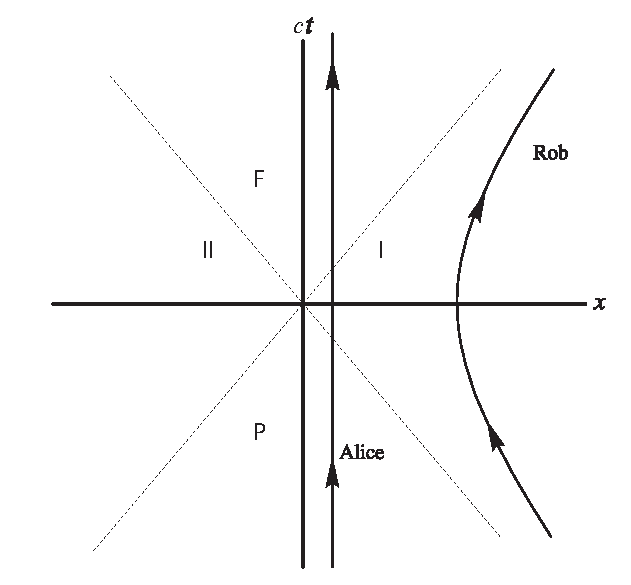
\includegraphics[width=.70\textwidth]{rin2}
\end{center}
\caption{Flat spacetime. Trajectories of an inertial (Alice) and accelerated (Rob) observer}
\label{rin2}
\end{figure}

Directly from \eqref{change} we see that for constant $\xi$ these coordinates describe hyperbolic trajectories in the spacetime whose asymptote is the light cone (as the observer accelerates his velocity tends to the speed of light, (i.e $ct\rightarrow x$). This means that a constantly accelerated observer follows trajectories such that $\xi=\text{const.}$ in the Rindler frame. However the observer for which these coordinates are his proper coordinates follows a particular trajectory:  To find its specific Rindler position we will use that all the Rindler observers are instantaneously at rest at time $t=0$ in the inertial frame, and at this time a Rindler observer with proper acceleration $a$ and, therefore, proper coordinates $(\xi,\tau)$ will be at Minkowskian position $x=c^2/a$. On the other hand, in this point $t=0\Rightarrow\xi=x$ instantaneously so, consequently, the constant Rindler position for this trajectory is $\xi= c^2/a$.

One can see that for accelerated observers an acceleration horizon appears: Any accelerated observer would be restricted to either region I or II of the spacetime. We will see in chapter \ref{blackhole1} that this horizon is locally very similar to an event horizon. The appearance of acceleration horizons is responsible for the Unruh effect \cite{Unruh}, as we will see in chapter \ref{tue}.  

A quick inspection reveals that the Rindler coodinates defined in \eqref{change} do not cover the whole Minkowski spacetime. Actually, these coordinates only cover the right wedge of the spacetime (Region I in Figure \ref{rin2}). This is so because an eternally  accelerated observer is always restricted to either region I or II depending if he is accelerating or decelerating with respect to the Minkowskian origin.

In fact to map the complete Minkowski spacetime we need three more sets of Rindler coordinates,
\begin{equation}\label{changeII}
ct=-\xi \sinh\left(\frac{a\tau}{c}\right),\qquad x=-\xi\cosh\left(\frac{a\tau}{c}\right),
\end{equation}
for region II, corresponding to an observer decelerating with respect to the Minkowskian origin, and
\begin{equation}\label{changeFP}
ct=\pm\xi \cosh\left(\frac{a\tau}{c}\right),\qquad x=\pm\xi\sinh\left(\frac{a\tau}{c}\right)
\end{equation}
for regions F and P.

Notice that for both relevant regions (I and II), the coordinates $(\xi,\tau)$ take values in the whole domain $(-\infty,+\infty)$. Therefore, they admit completely independent canonical field quantisation procedures. 


\subsection{Field quantisation in Minkowski and Rindler coordinates}

For simplicity, imagine first an inertial observer (Alice) in a flat spacetime whose proper coordinates are the Minkowskian coordinates $(x,t)$. She wants to build a quantum field theory for a free massless scalar field. 

As explained in section \ref{scalarfieldq}, to build her Fock space she needs to find an orthonormal basis of solutions of the free massless Klein-Gordon equation in Minkowski coordinates. Of course, she can always use the positive energy plane wave solutions of the Klein-Gordon equation in her proper coordinates to build a complete set of solutions of this equation.

In this fashion the states $\ket{1_{\hat \omega}}_\text{M}=a^\dagger_{\hat
\omega,\text{M}}\ket{0}_\text{M}$ are free massless scalar field
modes, in other words, solutions of positive frequency $\hat\omega$
(with respect to the Minkowski timelike Killing vector $\partial_{
t}$) of the free Klein-Gordon equation:
\begin{align}\label{modmin}
\ket{1_{\hat\omega}}_\text{M}&\equiv u_{\hat\omega}^\text{M}\propto\frac{1}{\sqrt{2{\hat \omega}}}e^{-i {\hat \omega} \hat t},
\end{align}
where only the time dependence has been made explicit. The label $\text{M}$ just means that these states are expressed in the Minkowskian Fock space basis.

The field expanded in these modes takes the usual form \eqref{exp1}
\begin{equation}\label{minkexp12}
\phi=\sum_i \left(a_{\hat\omega_i,\text{M}}u_{\hat\omega_i}^\text{M}+a_{\hat\omega_i,\text{M}}^\dagger u_{\hat\omega_i}^{\text{M}*}\right),
\end{equation}
where we have eliminated redundant notation and M denotes that $u_{\hat\omega_i}^\text{M}$ and $a_{\hat\omega_i,\text{M}}$ are Minkowskian modes and operators.

An accelerated observer   can also define his vacuum and excited states
of the field. Actually, there are two natural vacuum states associated
with the positive frequency modes in regions $\text{I}$ and $\text{II}$
of Rindler spacetime. These are $\ket{0}_\text{I}$ and
$\ket{0}_{\text{II}}$, and subsequently we can define the field
excitations using Rindler coordinates $(\xi,\tau)$ as
\begin{align}\label{modrin}
\ket{1_\omega}_\text{I}&=a^\dagger_{\omega,\text{I}}\ket{0}_\text{I}
\equiv u_\omega^\text{I}\propto\frac{1}{\sqrt{2\omega}}e^{-i\omega  \tau},\nonumber\\
\ket{1_\omega}_{\text{II}}&=a^\dagger_{\omega,\text{II}}\ket{0}_\text{II}
\equiv u_\omega^\text{II}\propto\frac{1}{\sqrt{2\omega}}e^{i\omega  \tau}.
\end{align}
These modes are related by a spacetime reflection and only have support in regions I and II of the
Rindler spacetime respectively.

We can now expand the field \eqref{minkexp12} in terms of this complete set of solutions of the Klein-gordon equation in Rindler coordinates
\begin{equation}\label{rindexp1}
\phi=\sum_i \left(a_{\omega_i,\text{I}}u_{\omega_i}^\text{I}+a_{\omega_i,\text{I}}^\dagger u_{\omega_i}^{\text{I}*}+a_{\omega_i,\text{II}}u_{\omega_i}^\text{II}+a_{\omega_i,\text{II}}^\dagger u_{\omega_i}^{\text{II}*}\right).
\end{equation}

Expressions \eqref{minkexp12} and \eqref{rindexp1} are exactly equal and therefore Minkowskian modes can be expressed as function of Rindler modes by means of the Klein-Gordon scalar product \eqref{KGsc}
\begin{equation}
u_{\hat\omega_j}^\text{M}=\sum_i\left[(u_{\hat\omega_j}^\text{M},u_{\omega_i}^\text{I})u_{\omega_i}^\text{I}-
(u_{\hat\omega_j}^{\text{M}},u_{\omega_i}^{\text{II}*})u_{\omega_i}^\text{II*}+(u_{\hat\omega_j}^\text{M},u_{\omega_i}^\text{II})
u_{\omega_i}^\text{II}-(u_{\hat\omega_j}^{\text{M}},u_{\omega_i}^{\text{I}*})u_{\omega_i}^\text{I*}\right].
\end{equation}
Notice that we have taken into account the properties \eqref{orto}, and one has to be very careful with the signs given that $(u^*_i,u^*_j)=-\delta_{ij}$.

If we now define Bogoliubov coefficients as
\begin{equation}\label{bogo11}
\alpha^{\Sigma}_{ij}=\left(u_{\hat\omega_i}^{\text{M}},u_{\omega_j}^\Sigma\right),
\qquad\beta^{\Sigma}_{ij}=-\left(u_{\hat\omega_i}^{\text{M}},u_{\omega_j}^{\Sigma*}\right),
\end{equation}
where $\Sigma$ can take the values I and II, we have that
\begin{equation}\label{minkowskirindlerexp}
u_{\hat\omega_j}^\text{M}=\sum_i\left(\alpha^{\text{I}}_{ji}u_{\omega_i}^\text{I}+
\beta^{\text{II}}_{ji}u_{\omega_i}^\text{II*}+\alpha^{\text{II}}_{ji}
u_{\omega_i}^\text{II}+\beta^{\text{I}}_{ji}u_{\omega_i}^\text{I*}\right).
\end{equation}
We would like to know how the creation and annihilation operators in the Minkowski basis are related to operators in the Rindler bases. Since we know that $a_{\omega_i,\text{M}}=(\phi,u_{\omega_i}^\text{M})$, if we write $\phi$ in Rindler basis \eqref{rindexp1} we can readily obtain
\begin{equation}\label{temporary1}
a_{\hat\omega_i,\text{M}}=\sum_j\left[(u_{\omega_j}^\text{I},u_{\hat\omega_i}^\text{M})
a^{\phantom{\dagger}}_{\omega_j,\text{I}}+(u_{\omega_j}^{\text{I}*},u_{\hat\omega_i}^\text{M})
a^\dagger_{\omega_j,\text{I}}+(u_{\omega_j}^\text{II},u_{\hat\omega_i}^\text{M})
a^{\phantom{\dagger}}_{\omega_j,\text{II}}+(u_{\omega_j}^{\text{II}*},u_{\hat\omega_i}^\text{M})
a^\dagger_{\omega_j,\text{II}}\right).
\end{equation}
Using the properties of the KG product
\begin{equation}\label{KGproperties}(u_1,u_2)=(u_2,u_1)^*\qquad(u_1^*,u_2^*)=-(u_2,u_1)\end{equation}
we can write \eqref{temporary1} in terms of the Bogoliubov coefficients \eqref{bogo11} as 
\begin{equation}
a_{\hat\omega_i,\text{M}}=\sum_j\left(\alpha^{\text{I}*}_{ij}
a^{\phantom{\dagger}}_{\omega_j,\text{I}}-\beta^{\text{I}*}_{ij}
a^\dagger_{\omega_j,\text{I}}+\alpha^{\text{II}*}_{ij}
a^{\phantom{\dagger}}_{\omega_j,\text{II}}-\beta^{\text{II}*}_{ij}
a^\dagger_{\omega_j,\text{II}}\right).
\end{equation}

A completely analogous reasoning can be followed for the case of a Dirac field, with some differences that will be deeply analysed in chapter \ref{sma} of this thesis. Where we will also go through the computation of the coefficients \eqref{bogo11}.

For now and for the sake of this introduction let us say that the vacuum state in the Minkowskian basis can be expressed as a two mode squeezed state in the Rindler basis \cite{Takagi, Alicefalls,NavarroSalas}. Namely, for the scalar case considered in this introduction
\begin{equation}\label{scalarvacuum1}
\ket{0}_{\text{M}}=\frac{1}{\cosh r}\sum_{n=0}^\infty \tanh^n r_{\text{b},\omega} \ket{n}_{\text{I}}\ket{n}_{\text{II}}.
\end{equation}
where\footnote{The label b stands for `bosonic', this parameter has a different definition for fermionic and bosonic fields as we will see in section \ref{probexcitations}}
\begin{equation}\label{rbos1}
r_{\text{b},\omega}=\operatorname{atanh} \left[\exp\left(-\frac{\pi c\omega }{a}\right)\right].
\end{equation}

\section{The Unruh effect}\label{tue}

In the 70s Fulling, Davies and Unruh realised that the impossibility to map the whole Minkowski spacetime with only one set of Rindler coordinates has strong implications when accelerated and inertial observers describe states of a quantum field. Namely, the description of the vacuum state of the field in the inertial basis as seen by accelerated observers has a non-zero particle content. 

In very plain words, the Unruh effect is the fact that while inertial observers `see' the vacuum state of the field, an accelerated observer would `see' a thermal bath whose temperature is proportional to his acceleration.

Different approaches to this well-known effect can be found in multiple textbooks (let us cite \cite{Wald2,Birrell,NavarroSalas} as a token). However, in this section, we will provide a not so common but rather simple derivation of the effect in a way that will be useful in order to clearly present a feature of spacetime with horizons which turns out to be relevant when it comes to study entanglement.

Imagine that an inertial observer, Alice, is observing the vacuum state of a scalar field. Now imagine an accelerated observer, called Rob, who wants to describe the same quantum field state by means of his proper Fock basis. The first step we need to take is to change the vacuum state from the Fock basis build from solutions to the Klein-Gordon equation in Minkowskian coordinates \eqref{modmin} to the Fock basis build from solutions of the KG equations in Rindler coordinates \eqref{modrin}. This gives us equation \eqref{scalarvacuum1} which we presented in the section above.

The state \eqref{scalarvacuum1} is a pure state. However, the accelerated observer is restricted to either region I or II of the spacetime due to the appearance of an acceleration horizon (as shown in Figure \ref{rin2}), and, since both regions are causally disconnected, Rob has no access to the modes which have support in the opposite wedge of the spacetime. This is a key point to analyse information matters. 

This means that the quantum state accessible for Rob is no longer pure,
\begin{equation}
\rho_{\text{R}}=\tr_{\text{II}}\left(\proj{0}{0}\right)=\sum_{k}\bra{k}_{\text{II}}\ket{0}_\text{M}\bra{0}_\text{M}\ket{k}_{\text{II}}.
\end{equation}
Substituting $\ket{0}$ by its Rindler basis expression \eqref{scalarvacuum1} we have that
\begin{equation}
\rho_{\text{R}}=\frac{1}{\cosh^2 r_{\text{b},\omega}}\sum_k\sum_{n,m}\tanh^{m+n}r_{\text{b},\omega}\bra{k}_{\text{II}}\ket{n}_\text{I}\ket{n}_{\text{II}}\bra{m}_\text{I}\bra{m}_{\text{II}}\ket{k}_{\text{II}},
\end{equation}
which leads to
\begin{equation}\label{thermal}
\rho_{\text{R}}=\frac{1}{\cosh^2 r_{\text{b},\omega}}\sum_n\tanh^{2n}r\ket{n}_\text{I}\bra{n}_\text{I},
\end{equation}
which is a thermal state.

Indeed, if we compute the particle counting statistics that the accelerated observer would see we obtain
\begin{equation}
\langle N_{\omega,\text{R}}\rangle=\tr_{\text{I}}\left(\rho_\text{R}\,a^\dagger_{\omega,\text{I}}a_{\omega,\text{I}}\right)=\frac{1}{e^{2\pi c/\omega a}-1},
\end{equation}
which is a Bose-Einstein distribution with temperature
\begin{equation}
T_\text{U}=\frac{\hbar a}{2\pi K_\text{B}},
\end{equation}
which is nothing but the Unruh temperature.

Rob observes a thermal state\footnote{Note that thermal noise is only observed in the 1+1 dimensional case. In higher dimension Rob would observe a noisy distribution, very similar to a thermal one, but with different prefactors \cite{Takagi}. This is called the Rindler noise.} because he cannot see modes with support in region II due to the presence of an acceleration horizon. This is a very important point that will play a fundamental role in some of the results presented in this thesis. 

As we will see in chapters \ref{blackhole1} and \ref{stellarcollapse} this effect is closely related with the Hawking effect and the Hawking radiation emitted in a stellar collapse process.


\section[Bogoliubov transformations in non-stationary scenarios]{Bogoliubov transformations in non-stationary\\ scenarios}\label{nonstaint}

We have mentioned in previous sections the difficulty of carrying out the field quantisation when the spacetime is not stationary. However, there are some very interesting scenarios in which the spacetime is not stationary but posses stationary asymptotic regions. This is the case of some models of expansion of the Universe \cite{dun1} or the stellar collapse and formation of black holes \cite{NavarroSalas}. As part of the thesis deals with quantum information problems   in such scenarios, an introduction to field quantisation in this context is in order.

Consider a spacetime which has asymptotic stationary regions in the past and in the future. We will call them `in' and `out' respectively.

The existence of these regions can be used to give a particle interpretation to the solutions of the field equations. Namely, we can build two different complete sets of solutions of the Klein-Gordon equation, the first one $\{u_{\hat\omega_j}^{\text{in}}\}$ made of modes that have positive frequency $\hat\omega_j$ with respect to the inertial time in the asymptotic past. The second set $\{u_{\omega_j}^{\text{out}}\}$ would consist of modes that have positive frequency $\omega_j$ with respect to the inertial time in the future.

In this fashion we can now expand the quantum field in terms of either the first or the second complete set of modes
\begin{equation}\label{minkexp1}
\phi=\sum_i \left(a_{\hat\omega_i,\text{in}}u_{\hat\omega_i}^\text{in}+a_{\hat\omega_i,\text{in}}^\dagger u_{\hat\omega_i}^{\text{in}*}\right)=\sum_i \left(a_{\omega_i,\text{out}}u_{\omega_i}^\text{out}+a_{\omega_i,\text{out}}^\dagger u_{\omega_i}^{\text{out}*}\right).
\end{equation}

Moreover, since both set of modes are complete, one can also expand one set of modes in terms of the other by means of the Klein-Gordon scalar product
\begin{align}\label{modinout1}
u^{\text{in}}_{\hat\omega_j}&= \sum_i \left[(u_{\hat\omega_j}^{\text{in}},u_{\omega_i}^{\text{out}})u_{\omega_i}^{\text{out}}-(u_{\hat\omega_j}^{\text{in}},u_{\omega_j}^{\text{out}*})u_{\omega_j}^{\text{out}*}\right],\\
u^{\text{out}}_{\omega_j}&= \sum_i \left[(u_{\omega_j}^{\text{out}},u_{\hat\omega_i}^{\text{in}})u_{\hat\omega_i}^{\text{in}}-(u_{\omega_j}^{\text{out}},u_{\hat\omega_i}^{\text{in}*})u_{\hat\omega_i}^{\text{in}*}\right].
\end{align}
Let us define Bogoliubov coefficients as
\begin{equation}
\alpha_{ij}=(u_{\omega_i}^{\text{out}},u_{\hat\omega_j}^{\text{in}}),\qquad \beta_{ij}=-(u_{\omega_i}^{\text{out}},u_{\hat\omega_j}^{\text{in}*}),
\end{equation}
then, using the properties \eqref{KGproperties} we can rewrite \eqref{modinout1} as
\begin{align}\label{modinout2}
u^{\text{in}}_{\hat\omega_i}&= \sum_j \left[\alpha_{ji}^{*}u_{\omega_j}^{\text{out}}-\beta_{ji}u_{\omega_j}^{\text{out}*}\right],\\
u^{\text{out}}_{\omega_j}&= \sum_i \left[\alpha_{ji}u_{\hat\omega_i}^{\text{in}}+\beta_{ji}u_{\hat\omega_i}^{\text{in}*}\right].
\end{align}

Now, we can expand the particle operators associated with one basis in terms of operators of the other basis. To do this we use the fact that $a_{\hat\omega_i,\text{in}}=(\phi,u_{\hat\omega_j}^{\text{in}})$ and $a_{\omega_i,\text{out}}=(\phi,u_{\omega_j}^{\text{out}})$, after some trivial computations and use of the properties of the scalar product we obtain
\begin{align}
\label{uno1}a_{\hat\omega_i,\text{in}}&=\sum_j \left(\alpha_{ji} a_{\omega_j,\text{out}}+\beta_{ji}^* a_{\omega_j,\text{out}}^\dagger\right),\\
a_{\omega_i,\text{out}}&=\sum_j \left(\alpha^*_{ij} a_{\hat\omega_j,\text{in}}-\beta_{ij}^* a_{\hat\omega_j,\text{out}}^\dagger\right).
\end{align}

Now let us consider the vacuum state in the asymptotic past region $\ket0_{\text{in}}$, which fulfils $a_{\hat\omega_i,\text{in}}\ket0_{\text{in}}$ for all $\hat\omega_i$. One could ask how that state evolves subject exclusively to the gravitational interaction, in other words, we want to know the form of the state $\ket0_{\text{in}}$ in the basis of solutions of the KG equation in the asymptotic future.

To do this we will take advantage of the fact that  $a_{\hat\omega_i,\text{in}}\ket0_{\text{in}}=0$, if we substitute $a_{\hat\omega_i,\text{in}}$ in terms of out operators using equation \eqref{uno1} we obtain that
\begin{equation}\label{condit}
\sum_j \left(\alpha_{ji} a_{\omega_j,\text{out}}+\beta_{ji}^* a_{\omega_j,\text{out}}^\dagger\right)\ket{0}_\text{in}=0.
\end{equation}

 
We can assume a general form for the state $\ket0_{\text{in}}$ in terms of the out Fock basis as a sum of its n-particle amplitudes
\begin{equation}\label{ansatz1}
\ket{0}_{\text{in}}= C\ket{0}_{\text{out}}+C^{j_1}\ket{\Psi}_{j_1}+C^{j_1,j_2}\ket{\Psi}_{j_1,j_2}+\dots+C^{j_1,\dots,j_n}\ket{\Psi}_{j_1,\dots,j_n}+\dots
\end{equation}
where each component has the form
\begin{equation}
C^{j_1,\dots,j_n} \ket{\Psi_n}_{j_1,\dots,j_n}=\sum_{j_1,\dots,j_n} C^{j_1,\dots,j_n} a_{\omega_{j_1},\text{out}}^\dagger\dots a_{\omega_{j_n},\text{out}}^\dagger\ket{0}_\text{out}.
 \end{equation}
 

Substituting the ansatz \eqref{ansatz1} in \eqref{condit} we obtain an infinite set of conditions for the coefficients $C^{j_1,\dots,j_n}$. First of all, for $C^{j}$ we see that the zero particle component of equation \eqref{condit}  can only be obtained from the annihilator acting on the 1-particle component of \eqref{ansatz1} state this gives the condition
\begin{equation}\label{coefcond1}
\sum_j\alpha_{j i}C^j=0\Rightarrow C^j= 0.
\end{equation} 

Now, the $n$-particle component ($n>0$) of equation \eqref{condit} is obtained by the annihilator acting  on the $n+1$ particle component of \eqref{ansatz1} and the creator acting on the $n-1$ particle component of \eqref{ansatz1}, therefore we know that the coefficients $C^{j_1,\dots,j_{n+1}}$ can be written as functions of the coefficients $C^{j_1,\dots,j_{n-1}}$ allowing us to find a recurrence rule to write all the coefficients as funcions of $C$ (the vacuum coefficient).

This, together with \eqref{coefcond1}, means that the `in' vacuum evolves to a state in the asymptotic future that does not have components of an odd number of particles and that the coefficients of even components in \eqref{ansatz1} are related pairwise. 

To find the form of this coefficients we take advantage of the invertibility of the Bogoliubov coefficient matrix $\alpha_{ij}$ and therefore given arbitrary $C_j$ and $D_j$ the following identity holds
\begin{equation}\label{inve}
\sum_j\left(\alpha_{j i}C_j+\beta_{ji}^*D_j\right)=0\Rightarrow C_k=-\sum_{ij}\beta^*_{ji}\alpha_{ ik}^{-1}D_j.
\end{equation}

After some basic but lengthy algebra we obtain that the vacuum state in the asymptotic past is expressed in the basis of modes in the asymptotic future as
\begin{equation}\label{dynoresult}
\ket{0}_\text{in}=C\exp\left(-\frac12\sum_{ijk}\beta^*_{ik}\alpha_{ kj}^{-1}a_{\omega_{i},\text{out}}^\dagger a_{\omega_{j},\text{out}}^\dagger\right)\ket{0}_\text{out}.
\end{equation}
C is obtained imposing the normalisation of the state.

This proves that if $\beta_{ij}$ is different from zero one would observe particle production as a consequence of time evolution under the interaction with the gravitational field. 

\section{The problem of field excitations\footnote{E. Mart\'in-Mart\'inez, L.J. Garay, J. Le\'on. Phys. Rev. D 82, 064006 (2010)} \footnote{D. \!
Bruschi,\! J. Louko,\! E. Mart\'in-Mart\'inez,\! A. Dragan,\! I. Fuentes,\! Phys.\! Rev.\! A 82,\! 042332 (2010)}}\label{probexcitations}

Most of the work regarding field entanglement in non-inertial frames before this thesis has made use of what was called the ``single mode approximation'' \cite{Alsingtelep,AlsingMcmhMil} in order to build the excited states of the field and transform them to the Rindler basis. As part of the results presented in this thesis we will see that such approximation was flawed and cannot be used as it was first presented. However, this does not mean that the previous works are wrong and not useful, but that they need reinterpretation.


It is obvious from \eqref{minkowskirindlerexp} that a single frequency Minkowski mode does not correspond to a monochromatic mode when it is transformed into the Rindler basis. In other words, a monochromatic field excitation in the Minkowskian basis transforms to a non-monochromatic field excitation from the perspective of an accelerated observer.

However, until 2010, all the previous studies analysing entanglement in a general relativisitc context employed the so-called single mode approximation.  This approximation, which was introduced in \cite{Alsingtelep,AlsingMcmhMil}, has been extensively used in the literature not only in discussions concerning entanglement but also in other relativistic quantum information scenarios, for example, among many others \cite{Alicefalls,AlsingSchul,Bradler,highdim,chapucilla,chapucilla2,Shapoor,matsako,Ditta,Geneferm,DiracDiscord}. 

Such approximation invokes that a single Minkowski mode transforms to a peaked distribution of Rindler modes and, therefore, one can approximate a single  Minkowski mode by means of a single Rindler mode; but this assumption is wrong. As we have mentioned above, the distribution of Rindler modes that corresponds to a single frequency Minkowski mode is not peaked, but highly non-monochromatic.

But there are specific bases which have the property of having diagonal Bogoliubov coefficient matrices. We will see that if we work in one of these bases we obtain results that are are computationally equivalent to those made under the single mode approximation. Now we proceed to build such a basis.

There exist an infinite number of orthonormal bases
that define the same vacuum state, namely the Minkowski vacuum
$\ket{0}_\text{M}$, which can be used to expand the solutions of the
Klein-Gordon equation.

 More explicitly, since the modes
$u^\text{M}_{\hat\omega_i}$ have positive frequency, any complete set
made out of independent linear combinations of these modes only
(without including the negative frequency ones
$u^{\text{M}*}_{\hat\omega_i}$) will define the same vacuum
$\ket{0}_\text{M}$.

Specifically, as described in e.g. Refs. \cite{Unruh,Takagi,Birrell} and
explicitly constructed in chapter \ref{sma}, there exists an orthonormal basis
$\{\psi_{\omega_j}^\text{M}, \psi'^{\text{M}}_{\omega_j}\}$ determined by certain linear
combinations of monochromatic positive frequency modes 
$u^\text{M}_{\hat\omega_i}$:
\begin{equation}\label{modopsi}
\psi^\text{U}_{\omega_j}=\sum_i C_{ij}\, u_{\hat\omega_i}^\text{M},\qquad \psi'^{\text{U}}_{\omega_j}=\sum_i C'_{ij}\, u_{\hat\omega_i}^\text{M} 
\end{equation}
 such that the Bogoliubov coefficients that relate this basis
 $\{\psi_{\omega_j}^\text{U},\psi'^{\text{U}}_{\omega_j}\}$  and the Rindler basis
 $\{u^\text{I}_{\omega_i},u^\text{II}_{\omega_i}\}$ have the following form:
 \begin{align}\label{bogo1}
\hat\alpha^{\text{I}}_{ij}
&=\left(\psi_{\omega_j}^\text{U},u_{\omega_i}^\text{I}\right)=\cosh r_{\text{b},\omega_i}\,\delta_{ij},
\nonumber\\
\hat\alpha^{\text{II}}_{ij}
&=\left(\psi_{\omega_j}^\text{U},u_{\omega_i}^{\text{II}}\right)=0,\nonumber\\
\hat\beta^{\text{I}}_{ij}
&=-\left(\psi_{\omega_j}^{\text{U}},u_{\omega_i}^{\text{I}*}\right) = 0,
\nonumber\\
\hat\beta^{\text{II}}_{ij}&=-\left(\psi_{\omega_j}^{\text{U}},u_{\omega_i}^{\text{II}*}\right)= \sinh r_{\text{b},\omega_i}\,\delta_{ij},
\end{align}
and analogously for $\hat\alpha'^{\text{I,II}}_{ij}$ and $\hat\beta'^{\text{I,II}}_{ij}$ interchanging the labels $\text{I}$ and $\text{II}$ in the formulas above. In this expressions
\begin{equation}\label{defr1}
\tanh r_{\text{b},\omega_i}=\exp(-\pi c {\omega_i }/{a}),
\end{equation}
and the label $\text{s}$ in $r_{\text{b},\omega_i}$ has been introduced to
indicate that we are dealing with a scalar field. %In this expression and in what follows, we will use Planck units ($\hbar=c=G=1$).

In this fashion a mode $\psi_{\omega_j}^\text{U}$ (or a mode $\psi'^{\text{U}}_{\omega_j}$) expands only in
terms of mode of frequency $\omega_j$ in Rindler regions
$\text{I}$ and $\text{II}$ and for this reason we have labeled $\psi_{\omega_j}^\text{U}$ and $\psi'^{\text{U}}_{\omega_j}$  with the frequency $\omega_j$ of the corresponding Rindler modes. In other words, we can express a given
monochromatic Rindler mode of frequency $\omega_j$   as a linear
superposition of the single Minkowski modes $\psi_{\omega_j}^{\text{U}}$ and $\psi'^{\text{U}*}_{\omega_j}$ or as a polychromatic combination of the
positive frequency Minkowski modes $u^\text{M}_{\hat\omega_i}$ and
their conjugates. These modes \eqref{modopsi} are nothing but a specific choice of the so-called Unruh modes \cite{Wald2,Birrell,NavarroSalas}. We will study this in detail in section \ref{sec3m7}.

Let us denote ${a_{\omega_j,\text{U}}}$ and $a_{\omega_j,\text{U}}^\dagger$ the
annihilation and creation operators associated with modes
$\psi^\text{U}_{\omega_j}$ (analogously we denote ${a'_{\omega_j,\text{U}}}$ and $a_{\omega_j,\text{U}}'^\dagger$ the ones associated with modes $\psi'^{\text{U}}_{\omega_i}$). The Minkowski vacuum
$\ket0_\text{M}$, which is annihilated by all the Minkowskian operators
$a_{\hat \omega_i,\text{M}}$, is also annihilated by all the operators
$a_{\omega_j,\text{U}}$ and $a_{\omega_j,\text{U}}'$, as we already mentioned. This comes out because any
combination of Minkowski annihilation operators annihilates the
Minkowskian vacuum.

Due to the Bogoliubov relationships \eqref{bogo1} being diagonal, each annihilation
operator $a_{\omega_i}$ can be expressed as a combination of Rindler
particle operators of only one Rindler frequency  $\omega_i$:
\begin{equation}\label{buenmod}
a_{\omega_i,\text{U}}=\cosh r_{\text{b},\omega_i}\, a^{\phantom{\dagger}}_{\omega_i,\text{I}}-
\sinh r_{\text{b},\omega_i}\,a^\dagger_{\omega_i,\text{II}},
\end{equation}
and analogously for $a'_{\omega_i}$ interchanging the labels I and II.

An analogous procedure can be carried out for fermionic fields (e.g. Dirac
fields). We can use linear combinations of monochromatic solutions of the
Dirac equation $\psi^\text{U}_{\omega_i,\sigma}$ and $\bar
\psi^\text{U}_{\omega_i,\sigma}$ (and their primed versions) built in the same fashion as for scalar
fields:
%\begin{align}\label{modopsif}
%\psi^\text{M}_{\omega_j,\sigma}=\sum_i D_{ij}\, u_{\hat\omega_i,\sigma}^\text{M},
%& \bar \psi^\text{M}_{\omega_j,\sigma}=\sum_i E_{ij}\, v_{\hat\omega_i,\sigma}^\text{M},\\
%\psi'^{\text{M}}_{\omega_j,\sigma}=\sum_i D'_{ij}\, u_{\hat\omega_i,\sigma}^\text{M},
%& \bar\psi'^{\text{M}_{\omega_j,\sigma}=\sum_i E'_{ij}\, v_{\hat\omega_i,\sigma}^\text{M},
%\end{align}
\begin{align}\label{modopsif}
\psi^\text{U}_{\omega_j,\sigma}=\sum_i D_{ij}\, u_{\hat\omega_i,\sigma,\text{M}}^{+},
&\qquad \bar \psi^\text{U}_{\omega_j,\sigma}=\sum_i E_{ij}\, u_{\hat\omega_i,\sigma,\text{M}}^{-},\nonumber\\
\psi'^{\text{U}}_{\omega_j,\sigma}=\sum_i D'_{ij}\, u_{\hat\omega_i,\sigma,\text{M}}^{+},
& \qquad\bar\psi'^{\text{U}}_{\omega_j,\sigma}=\sum_i E'_{ij}\, u_{\hat\omega_i,\sigma,\text{M}}^{-},
\end{align}
where $u^+_{\hat\omega_i,\sigma,\text{M}}$ and
$u^-_{\hat\omega_i,\sigma,\text{M}}$ are respectively monochromatic
solutions of positive (particle) and negative (antiparticle) frequency $\pm\hat\omega_i$ of the
massless Dirac equation with respect to the Minkowski Killing time. The
label $\sigma$ accounts for the possible spin degree of freedom of the
fermionic field\footnote{Throughout this work we will consider that the
spin of each mode is in the acceleration direction and, hence, spin will not
undergo Thomas precession due to instant Wigner rotations
\cite{AlsingSchul,Jauregui}.}.

The coefficients of these combinations are such that for the modes
$\psi_{\omega_i,\sigma}$ and $\bar \psi_{\omega_i,\sigma}$ the
annihilation operators are related with the Rindler ones by means of the
following Bogoliubov transformations:
\begin{eqnarray}\label{Bogoferm2}
\nonumber c_{{\omega_i},\sigma,\text{U}}&=&\cos{r_{\text{f},\omega_i}}\,c_{{\omega_i},
\sigma,\text{I}}-\sin r_{\text{f},\omega_i}\,d^\dagger_{{\omega_i},-\sigma,\text{II}},\\*
d_{{\omega_i},\sigma,\text{U}}^\dagger&=&\cos{r_{\text{f},\omega_i}}\,d^\dagger_{
{\omega_i},\sigma,\text{II}}+\sin r_{\text{f},\omega_i}\,c_{{\omega_i},-\sigma,\text{I}},
\end{eqnarray}
and analogously for $c'_{\omega_i,\text{U}}$ and $d'^\dagger_{\omega_i,\text{U}}$ interchanging the labels I and II, where \footnote{Although convenient, the notation for the parameters $r_{\text{f},\omega_i}$ and $r_{\text{b},\omega_i}$ can sometimes be excessive in the long and complex expressions that will appear throughout this thesis. Consequently, we will drop the labels b,f or $\omega_i$ to ease notation whenever there can be no ambiguity or confusion.}
\begin{equation}\label{defr}
\tan r_{\text{f},\omega_i}=\exp(-\pi c{{\omega_i}}/{a}).
\end{equation}
Here $c_{{\omega_i},\sigma}$, $d_{{\omega_i},\sigma}$ represent the
annihilation operators of modes $\psi^\text{U}_{\omega_i,\sigma}$ and
$\bar
\psi^\text{M}_{\omega_i,\sigma}$ for particles and antiparticles respectively. 
The label $\text{d}$ in $r_{\text{f},\omega_i}$ has been introduced to indicate
Dirac field. The specific form for $\psi^\text{U}_{\omega_i,\sigma}$
and $\bar
\psi^\text{U}_{\omega_i,\sigma}$ as a linear combination of monochromatic
solutions of the Dirac equation is given later in section \ref{secferme}, and can be also seen, for instance, in
\cite{Jauregui,chinada} among many other references. Notice again that,
although we are denotating $a_{\omega_i,\text{U}},
c_{\omega_i,\sigma,\text{U}}, d_{\omega_i,\sigma,\text{U}}$ the operators associated
with Minkowskian Unruh modes, those modes are not monochromatic, but a
linear combination of monochromatic modes given by \eqref{modopsi} and
\eqref{modopsif}.

To discuss fundamental issues and not an specific
experiment, there is no reason to adhere to a specific basis. Specifically,
if we work in the bases \eqref{modopsi} and
\eqref{modopsif} for Minkowskian modes we do
not need to carry out the single mode approximation.


We will work in this basis in  part \ref{part1} of this thesis. This will be useful to extend and compare some of the results obtained here with previous works that made use of the single mode approximation. In part \ref{part2} we will discuss the problems of the single mode approximations and how to relax it, presenting the most general way to work with Unruh modes and the new and interesting results that appear when we go beyond a specific choice of Unruh modes.







\cleardoublepage
